\documentclass[11pt]{article}

\usepackage{graphicx}
\graphicspath{{figures/}}

\usepackage{mathtools}
\usepackage{amssymb}
\usepackage{amsmath}
\DeclareMathOperator*{\argmin}{argmin}
\DeclareMathOperator*{\argmax}{argmax}

\usepackage{xcolor}
\usepackage{subfigure}
\usepackage{caption}

\usepackage[font=footnotesize,labelfont=bf]{caption}

\usepackage[T1]{fontenc}

\renewcommand{\rmdefault}{ppl}
\renewcommand{\sfdefault}{phv}
\renewcommand{\ttdefault}{pcr}
\renewcommand{\familydefault}{\sfdefault}
\newcommand{\norm}[1]{\left\lVert#1\right\rVert}

\usepackage{fancyhdr}
\fancypagestyle{firstpage}{\fancyhf{}\fancyhead[R]\fancyfoot{New York, \today}}
\fancypagestyle{plain}{\fancyhf{} \fancyhead[R]{\thepage}}
\renewcommand{\headrulewidth}{0pt}

\usepackage{geometry}
\geometry{letterpaper}
%\geometry{margin= 1 in}
\geometry{margin=2cm}

\renewcommand{\baselinestretch}{1.25}
\setlength{\parindent}{0in} 
\setlength{\parskip}{0.1in}

\renewcommand{\t}{\theta}
\newcommand{\td}{\tilde{\theta}}

\long\def\comment#1{}

\definecolor{darkblue}{rgb}{0.1,0,0.6}
\definecolor{green}{rgb}{0,1,0}
\newcommand{\cc}{\color{darkblue}}
\newcommand{\torevise}{\color{green}}
\newcommand{\mbf}{\mathbf}
\newcommand{\sbf}{\boldsymbol}
\begin{document}



% MANUSCRIPT
% title

\section*{\LARGE  Invariance and selectivity to spatial variables in deep neural networks and the brain }

% notes written by 
% layout
% title
% abstract
% intro
% results
% discussion

Margaret C Von Ebers\textsuperscript{1,3,4} and Xue-Xin Wei\textsuperscript{1,2,3,4}


1) Department of Neuroscience, The University of Texas at Austin\\
2) Department of Psychology, The University of Texas at Austin\\
3) Center for Perceptual Systems, The University of Texas at Austin\\
4) Center for Theoretical and Computational Neuroscience, The University of Texas at Austin

\section*{Abstract}
The mammalian hippocampus contains cognitive maps of the spatial environment. Various types of spatial cells, such as grid cells, place cells, head direction cells, border cells together form such maps.  Multiple recent studies suggest that, surprisingly, model units in deep vision-based networks are selective to locations as well as other spatial variables, despite that these networks receive only visual, but not spatial inputs. This challenges the dominant view that cognitive maps are constructed based on path integration process.  While these studies as well as most previous studies emphasize the selectivity of individual neurons to one or more spatial variables, the invariance to other spatial variables have not been systematically studied. We propose a new analysis framework to examine the contribution of a variable to the neuron's response variability. Applying this new framework to deep vision-based networks, we consistently found that ``place cells" identified in these networks are not invariant to head direction. 
To the contrary, our results on the tuning properties of hippocampus place cells and reveal that place cells are not only selective to location, but are also invariant to head direction. Thus, model units in deep nets exhibit drastically different coding properties compared to the place cells in rodents. 
Our results show that it is important to study their joint tuning properties in order to understand the selectivity and invariance of neural code. Our framework is general, and should be applicable to study the neural code in other domains, beyond spatial navigation. 

\newpage

{\bf A list of figures [need the higher resolution versions of the figures for the submission]}:


Fig. 1. (a) An illustration of the issue of computing marginal tuning when samples are correlated, using simulation. Refer to Section 2.1. We can generate several panels showing cases for which the two dimensions are (i) uncorrelated, (ii) modestly correlated; (iii) strongly correlated. (b) Using simulation to show that GLM failed to recover the ground truth, when the tuning for the two dimensions are not multiplicative. Refer to Section 2.1. %\textcolor{red}{XX: alternatively, we can show the GLM in later figures when we analyze the data/model.}

Fig. 2. Show that GLM can not properly capture the joint tuning



Fig. 3. (a) A schematic figure illustrate our estimation approach. (b) Show that method provide an unbiased estimate of the variance explained by individual variables with discrete sampling. %\textcolor{red}{XX: we can also consider adding an additional panel showing binning may cause a small positive bias when the data are collected based on continuous variables (e.g., MD \& HD).}

Fig. 4. Results on place cells in 2-D. (a) show some 3-D tuning curves of place cells (location times head direction). (b) Show the variance explained by the location and HD.
(c) a panel showing the decoding results on HD based on a cross-validated decoder, to show that the place cell population contains very little HD information. 

Fig. 5. Results on the HD cells. (a) show the 3-D HD cells (location time head direction). (b) Show the variance explained by the location and HD. (c) a panel showing the decoding results on HD based on a cross-validated decoder, to show that the HD population contain very little location information. Joint decoding or separate decoding?


Fig. 6. Results based on the CNN models. (a) Show a schematic of the model in Luo et al. (b) Plot some example marginal tuning curves and joint tuning. (d) Show quantification of contribution of location and HD using our method. 

Fig. 7. Results based on the predictive coder. (a) Show a schematic of the predictive network. (b) Plot some example marginal tuning curves and joint tuning. (d) Show quantification of contribution of location and HD using our method. 

Fig. 8. Decoupling the encoding of MD and HD in the head direction cells. (a) Show some example HD and MD tuning curves. (b) Show the joint tuning of the two. (c) A figure showing the quantification of the contribution of the two variables using our method. 

\newpage
\section{Introduction}

% discuss the neural tuning
Neural code is often studied by study the tuning property of individual neurons. Over the past few decades, neuroscientists have characterized the tuning properties of neurons in many brain areas in many different tasks. In visual cortex, it is known that many neurons are selective to orientation, direction, spatial and temporal frequency of the stimulus. In the hippocampus and interconnected brain areas such as entorhinal cortex and parahippocampus, various types of neurons were found and are selective to different spatial variables. Note that while some neurons are selective to one spatial variable, others may be tuned by multiple variables. 



% discuss the cognitive maps 
How the brain constructs maps of the environment represents a fundamental question in neuroscience. It is generally believed that spatial inputs (e.g., velocity input and head rotation) are needed, and the brain integrates such inputs to generate spatial maps. This hypothesis is often referred to as the path integration hypothesis. Models based on this idea have been proposed using attractor dynamics. More recently, it is shown that by optimizing recurrent networks to perform path integration, grid firing patterns can emerge after network training. Other sensory inputs are often important in the construction of the cognitive map. In particular, they have been thought to be important to form landmarks to recalibrate the spatial map. 

% discuss models of cognitive maps and the recent results
However, recent studies challenged this view. By studying deep network models constructed to solve pure visual tasks, it is argued that many model units in these neural network can exhibit spatial tuning properties similar to the spatial functional cell types observed in the hippocampus. These models provide new candidate models for studying the mechanisms of the origin of the spatial selectivity of the hippocampus neurons. They are particularly interesting because they do not involve 
any path integration process, unlike most prior models. 
Based on these models, it has also been argued that the spatial functional cell types may be supercilious as they may emerge as a natural consequence of complex network computation that may nothing to do with spatial cognition. 


When analyzing the tuning properties of an individual neuron, in particular the spatial tuning properties, one often relies on examining its tuning curve. For a given variable, one can estimate the firing rate of a neuron as the variable varies. This is called the tuning curve. When analyzing the tuning for multiple variables, two approached are often taken. The first approach is to compute the tuning curve for each variable separately. 
The second approach is to using a generalized linear model framework (GLM) to analyze the potentially ``mixed selectivity". One drawback of this framework is that it assumes that the joint tuning can be factorized into the product of the marginal tuning curves. Indeed, the spatial tuning properties of neurons in the hippocampus (as well as many other brain areas) were based on characterizing the selectivity of individual dimensions. However, these analysis were based on characterizing and comparing the tuning curves for individual stimulus variables, it remain unclear whether the tuning properties to the set of relevant stimulus variables are indeed similar for the network and the brain.


Here, we propose that it would be most informative to examine the joint tuning properties to multiple stimulus variables. This will provide a more unbiased characterization of the tuning properties. We first show that characterizing the tuning for one variable at a time is insufficient for describing the full tuning.
We devise a new analysis framework to analyze the selectivity and invariance of tuning to a given variable. Applying this framework to analyze the deep vision-based models and the hippocampus neural responses during a navigation task, we find there is both qualitative difference and large quantitative difference between the model and the brain. Our results demonstrate the limitation of the standard tuning curve based method and suggest new approaches to better understand the tuning properties of individual neurons.



% summarize what we did



\section{Results}

\subsection{Marginal tuning is insufficient to capture the joint tuning property}

For a given neuron, when only one variable (denoted as $x$) is considered, the tuning properties can be conveniently described by the tuning curve $f(x)$. The tuning curve quantifies the expected firing rate of a neuron for a given stimulus variable.
If another stimulus variable $y$ is also of interest, the tuning curve $g(y)$ can also be computed. Suppose that our goal is to understand whether this neuron is selectivity to $(x,y)$, one may attempt to examine the function $f(x)$ and $g(y)$ to see if one or both of them show strong selectivity. Suppose that $f(x)$ is a narrow Gaussian function, and $g(y)$ is completely flat, it is tempting to claim that this neuron is selective to variable $x$, and it is invariant to $y$. However, this interpretation may not be warranted. Fig. 1a illustrate one example. In this case, the response of the neuron is clearly not invariant to $y$, yet the marginal tuning on $y$ is flat. Variable $y$ still accounts for the variability of the neural response through its interaction with the encoding of $x$.

One can consider a more extreme example (see Fig. 1b). In this case, the tuning curves $f(x)$ and $g(y)$ are both flat. However, it would be clearly unreasonable to claim that this neuron is invariant or not selectivity to $x$ and $y$. When knowing the firing rate of the neuron, one can substantially narrow down the possible  values of $x, y$. The joint tuning of the both variable are strongly selective. However, their contribution are highly entangled that can not be revealed by the marginal tuning curves based on individual stimulus variable. 

There are certainly cases where it is possible to interpret the tuning properties of the neurons based on the marginal tuning curves. One such scenario is that the joint tuning can be factorized into the product of the marginal tuning curves for the individual stimulus variables, i.e., $h(x,y)=f(x)g(y)$. Fig. 1c illustrate one such scenario. In particular, if $g(y)$ is flat and $f(x)$ is not flat, one can conclude that this neuron is selective to $x$ and invariant to $y$.
There are indeed some evidence suggesting that for certain neurons and certain stimulus variables, there may be a multiplicative relationship between the joint tuning and the marginal tuning along individual dimensions [ref]. The popular GLM framework used in neural data analysis also make this assumption. Because in most applications of GLM, an exponential link function is assumed-- linearly adding responses in log of firing rates is equivalent to multiplying the tuning curves. 
However, in general this assumption needs to be tested experimentally. 

\begin{figure}[h!]
    \centering
    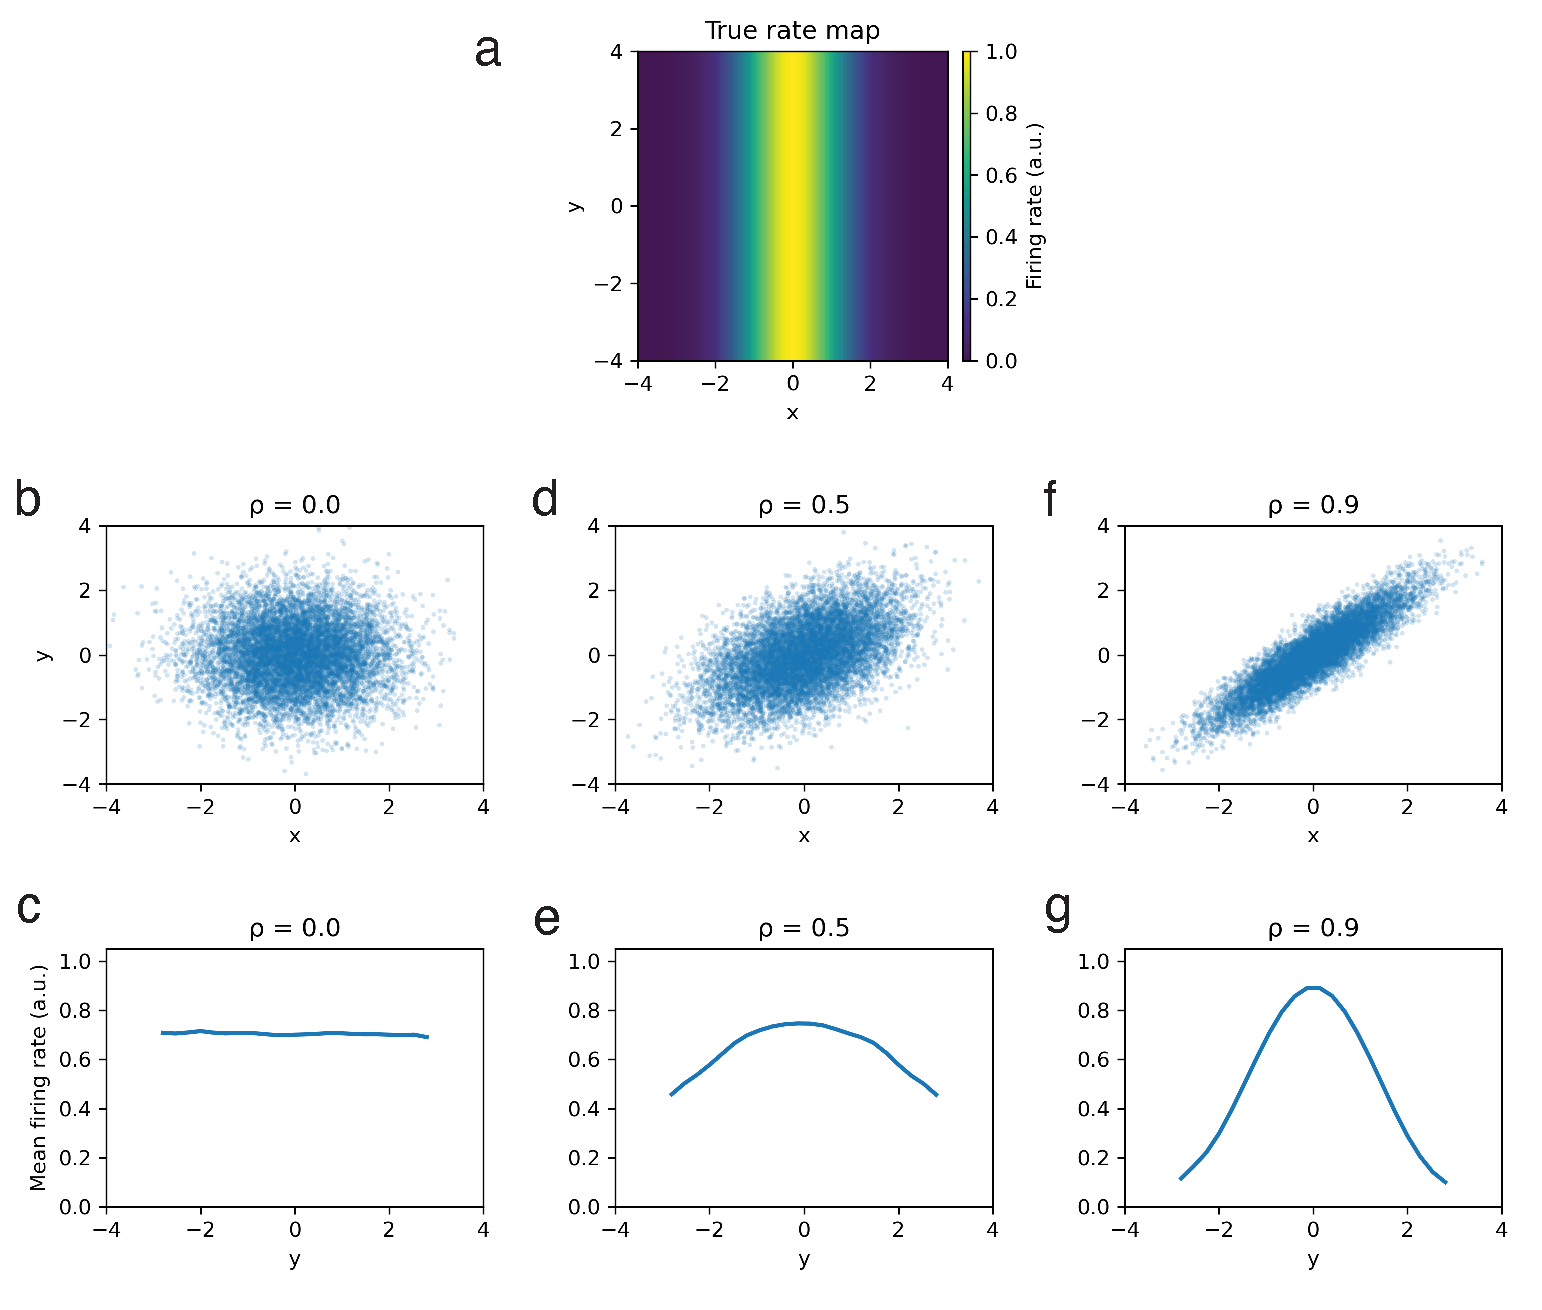
\includegraphics[width=0.8\textwidth]{Figures/CNN_fig1.pdf}
    \caption{\textbf{The joint tuning curve of a neural can not be adequately described by the marginal tuning.} }
    \label{fig:fig1}
\end{figure}



If a neuron is selective to multiple stimulus variables, this is often referred to as conjunctive tuning. More recently, ``mixed selectivity" is also used to describe the selectivity to multiple stimulus variables. If the multiplicative relationship between marginal and joint tuning holds, we will refer to it as linear mixing (because it is consistent with a GLM framework). Otherwise, we will refer to it as nonlinear mixing. 


The interpretation of marginal tuning curves is further complicated by the correlated sampling of the stimuli. Consider the case of studying the neural tuning of two correlated stimulus variables. Correlated stimulus variables are fairly common, in particular, when studying spatial navigation. One example of such correlated variables are the head direction and movement direction of the animal during navigation. Another example is the time and distance traveled when the animal is running on a linear track. Suppose that a neuron is select to one variable (say head direction), while invariant to the other variable (say movement direction). Fig. XX show example simulation results in this setting. 
It is evident that the marginal tuning curve on head direction is also narrowly tuned. This is due to biased sampling in the stimulus space. 

Assuming uniform sampling over $x$, the marginal tuning curve for $x$ is estimated to be
$$
\hat{f}(x) = \int p(y|x)h(x,y)dy = \int p(y|x)f(x) g(y)dy =f(x)\int p(y|x)g(y)dy
$$

%\textcolor{red}{Add a figure to demonstrate the problem of computing marginal tuning when samples are correlated.}

If $x$ and $y$ are independent, the procedure recovers $f(x)\int p(y)g(y)dy$, which is proportional to $f(x)$. Otherwise, due to the interaction in the $p(y|x)$ term, the estimated marginal tuning curve on $x$ will be affected by $g(y)$. 
%In the extreme case that only $y=x$ is sampled, the estimated tuning curve becomes $f(x)g(x)$.

Consider a special case where the neuron is invariant to $x$, i.e., $h(x,y)=h(y)$ is a narrow Guassian function. We further assume that only $y=x$ is sampled
$$
\hat{f}(x) = \int p(y|x)h(y)dy = \int \delta(y-x)h(y)dy=h(x).
$$
In this case, if we rely on computing the marginal tuning curves to infer the tuning properties, we would incorrectly conclude that the neuron is strongly tuned to $x$.




\begin{figure}[h!]
    \centering
    \includegraphics[width=0.8\textwidth]{Figures/CNN_fig_GLM.pdf}
    \caption{\textbf{The joint tuning curve may not be captured by the generalized linear model (GLM).} }
    \label{fig:fig1}
\end{figure}


An alternative approach would be to fit a GLM model to the neural response directly. To assess whether GLM can correctly identify the regime of correlated sampling, we generate simulated neural response from the model above, and fit GLM to the model responses.  We find that ...

%\textcolor{red}{Testing if GLM can recover the invariance for the second dimension in cases the neuron is only selective the first dimension and the stimulus sampling is biased.  }

%\textcolor{red}{Add a figure on GLM to show the model recovery with correlated sampling, and when the two dimensions are not multiplicative.}






\subsection{Analyze the invariance and selectivity of the joint tuning}

Our results above show, when analyzing the selectivity and invariance of the neural response properties, it is crucial to examine the joint tuning properties beyond the marginal tuning curves.
By only considering the marginal tuning, one may lead to misinterpretation of the structure of the code. 




How can we study the joint tuning properties of an individual neuron? To our knowledge, no systematic tools have been developed in the field. 
Practically, one simple procedure to get a sense of whether the neural response is invariant to a stimulus variable $x$ is to vary $x$ and examine the tuning for the remaining variables. If only two variables are considered, this amount to examine the tuning curve of $g(y)$ conditioned on different value of $x$. 
If the tuning curve for $y$ is invariant when changing $x$, one may conclude that the response of this neuron is invariant to variable $x$. Otherwise, the response of this neuron depends on variable $x$. In other words, variable $x$ contributes to the response variability of this neuron. It is important to note that such dependence may have many different forms depending on the problems and the neurons being studied. One particularly simple form of dependence is a gain change. That is, if varying $x$ leads to a multiplicative change of the tuning curves for $y$, the joint tuning for $x,y$ can be factorize into a product of the marginal tuning for $x$ and $y$.


\begin{figure}[h!]
    \centering
    \includegraphics[width=0.99\textwidth]{Figures/CNN_fig2.pdf}
    \caption{\textbf{The joint tuning curve of a neural can not be adequately described by the marginal tuning.} }
    \label{fig:estimation}
\end{figure}


To quantify the joint tuning to understand the contribution of individual variables as well as their nonlinear interactions, we develop a simple analysis approach based on the intuition described above. To quantify the contribution of variable $x$, we calculate the variability of the joint tuning that is not explained by the other variables. In the case of two variables, this is amount to the residual variability that is not explained by $y$. Similarly, one can calculate the contribution of $y$ via the variability that is not explained by $x$. Notably, unlike ANOVA for linear additive models, summing up the contribution of $y$ and $x$ may not equal to the total variance of the data. 

Practically, one challenge of applying this idea is the measurement noise. Consider a case mentioned above in which the neural response is completely invariant to variable $y$. Due to measurement noise (which could come from many sources), there will be residual variability in the estimate joint tuning curves that can not be explained by $x$. If one simply uses the residual variance to estimate the contribution of variable $y$, the true contribution will be over-estimated. Thus, it is important to properly take into account the impact of measurement noise. To do so, we develop a procedure to estimate the variability induced by noise by quantifying the variability across the joint tuning estimated from the two splits of the data. Our final estimate for the contribution of individual stimulus variables remove such noise-induced variability.

As a complementary approach to the non-parametric approach described above, we also considered a parametric approach by constructing models based on mixture of product of Gaussian functions. In the case of having only one mixture component, the model reduces to one that assume (i) the marginal tuning of the two variables are both Gaussian; (ii) a multiplicative interaction between the tuning to the two variables.
By incorporating multiple components, the model is more flexible than the standard GLM and allows more complex patterns of mixing of the tuning properties. In applications, one interesting question is whether models with multiple mixture components would outperform the standard one component model. Because each mixture component is parameterized by Gaussian function with only a few parameters, this mixture model remain feasible in fitting to limited amount of experimental data.

\subsection{Place cells are selective to location and invariant to head direction}

Leveraging our new framework, we analyze the neural responses in the hippocampus recorded when the rats were performing a navigation task in a two-dimensional open environment. This dataset were originally published in [ref]. We first computed the spatial firing rate maps for individual neurons. Consistent with the previous reports, we find that many neurons are selective to spatial location. Each neurons have one or more place fields. While it has been documented that most place cells were not tuned to head direction (also confirmed by our own analysis on marginal tuning of head direction), however, it was unclear whether the hippocampus neurons with place cells exhibit strong invariance to head direction. To investigate this question, we computed the joint tuning curve for location and HD. For each neuron, this results in a 3D heatmap. Indeed, visual inspection suggests that the neural response is invariant to HD. However, due to non-uniform sampling in the data, some combinations of HD\&location have few or no data. To address this question, we did two additional visualization. 

\begin{figure}[h!]
    \centering
    \includegraphics[width=0.99\textwidth]{Figures/CNN_fig_place.pdf}
    \caption{\textbf{Place cells in the rat hippocampus are selective to locations and largely invariant to head direction.} }
    \label{fig:PlaceCell}
\end{figure}

%\textcolor{red}{Add a figure on 3-D tuning curves of place cells, and add a figure to quantify variance explained by place and HD }

First, we plot the joint tuning for HD and x-axis of the 2-D environment. This analysis projects the 3D data onto 2-D subspace defined by HD and x-axis of location. If the neuronal response is invariant to HD, the heatmap should be dominated by vertical bar/stripe. This is indeed true for most neurons that were classified as place cells according to standard procedures used for analyzing place cells. 
Similar results hold when examining the joint tuning for HD and y-axis of the 2-D environment.

Second, we reduce the number of HD bins into 4 (each bin corresponds to one quadrant). For each HD bin, we computed the 2-D spatial firing rate map. Fig. XX shows one example neuron. As can been seen from the plots, the 2D place fields under different HD directions are highly consistent. We quantify the correlation between the different maps, and find the correlation to be... [Perform some quantification]
We reason that the deviation from a perfect correlation is due to noise in the neural response. If this is the case, we expect that the correlation between spatial maps conditioned on different HD should be dependent on the firing rate of the neuron. Examining the relationship between the correlation values of maps and the firing rate, we find that ...

Third, we quantify the contribution of the HD and 2-D location using the procedure we developed. We find that the ratio between the neural response variability explained by HD and that explained by the location is XX. 

Perform decoding analysis on HD. If tuning is invariant to HD, the decoding performance should be at chance level.


\begin{figure}[h!]
    \centering
    \includegraphics[width=0.99\textwidth]{Figures/CNN_fig_HD.pdf}
    \caption{\textbf{Head direction cells in the rat hippocampus are selective to head direction, and is largely invariant to location.} }
    \label{fig:HD}
\end{figure}

%\textcolor{red}{Head direction cells contain little information about space?}

%\textcolor{red}{Add a figure on the HD decoding results}

\subsection{Model units in CNNs exhibit entangled pattern of tuning}
While many prior studies suggest that path integration is important for the formation of cognitive maps in the brain, recent studies reported that place cell-like response in deep neural networks trained to perform vision tasks. XX analyzed the response of individual units in ResNet (pretrained on image classification tasks) in a spatial task. Specifically, they model the visual inputs of an virtual agent navigating in a 2-D open area that is similar to the typical environment for experiments done in rodents. Importantly, the network only receives visual input, and no velocity input. Surprisingly, they reported many neurons in the network throughout the layers exhibit place cell-like responses using methods that are similar to what were used in prior literature to analyze the hippcampus neurons in spatial tasks. They also analyze the tuning for HD and border.


\begin{figure}[h!]
    \centering
    \includegraphics[width=0.99\textwidth]{Figures/CNN_fig_CNN.pdf}
    \caption{\textbf{Model neurons in CNNs trained on image recognition tasks exhibit highly entangled tuning properties for location and head direction.} }
    \label{fig:CNN}
\end{figure}


%\textcolor{red}{Add some example neurons tuning curves, and the quantification using our method}

Importantly, XX only examined the marginal tuning for place and HD. It remains unclear whether the joint tuning for place and HD would be similar to that of hippocampus place cells. 
We hypothesize that while the model neurons may exhibit place fields when examining the marginal tuning for location, the model neurons may not exhibit invariance to HD as in hippocampal place cells. 

We first analyze the marginal tuning for location and HD. Indeed, we found that some neurons exhibit place fields in 2D space. This is similar to what was reported in XX. Ref XX also reported that many model units exhibit strong head direction tuning and a subset of neurons exhibit conjunctive place and HD tuning. Our own analysis suggests that few model units are tuned to HD and almost none of them are conjunctive place and HD cells. At the face value, this seems to suggest that the model units exhibit properties similar to real place cells in rodents. It is important to note that, according to our results above, it is necessary to examine the joint tuning of place and HD to better compare the two.

To investigate this question, we first visualize the 3D place and HD maps for the model units that have been classified as tentative place cells. These plots (see Fig. XX) suggests that the firing fields are highly scattered in the 3D space. Few neurons exhibit invariance to HD. Typically, the model unit only generate high activity with particular combinations of place and HD.

We also visualize the joint tuning of HD and the first dimension of space, and the joint tuning of HD and the second dimension of space. The results again show that the response of models units are not invariant to HD. 

We compute the location map for four different HDs, and then evaluate the correlation between these maps. We find that the correlation is ...
This is much smaller than what we found in hippocampus place cells.

We further quantify the variance of the firing rate map explained by HD and location and found that the two explain about similar amount of variability. This suggests that the tuning for HD and location are highly entangled. We compared these results to what we obtained from the rat hippocampus (see Fig. XX). 

We reason that this highly mixed code may due to that (i) the model units are encoding visual features, and (ii) the visual features in the environment are related to the HD and location in a complicated way. Only a particular combination of HD and location may result in the particular visual feature preferred by a model unit. To test this idea, we examine the model units in the first layer of the network for which their response properties can be easily interpreted using the receptive fields. In particular, we identify neurons with oriented receptive fields and examine their place and HD tuning. We find... 

We conclude that the model units were not encoding location per se, instead they form a high mixed code that represents particular combination of head direction and location. This code is qualitative and quantitative different from the place code in the rat hippocampus. 

One should be able to decode HD from the model response.

\subsection{Model units in networks constructed based on predict coding also exhibit entangled pattern of tuning}

We perform similar analysis on a different network that were trained on different task objectives. In ref XX, they trained neural network to predict the next frame of visual inputs for a navigation agent. They found place-cell-like representation in the later layer of the network. In their basic model, the head direction of the virtual agent is assumed to be fixed, which is not realistic. It is possible to modify their model framework to make head direction variable. We trained this augmented version of the model and examine the model units throughout the network. 


\begin{figure}[h!]
    \centering
    \includegraphics[width=0.99\textwidth]{Figures/CNN_pred_ver2.pdf}
    \caption{\textbf{Model neurons in deep networks trained to predict the next image framework also exhibit highly entangled tuning properties for location and head direction.} }
    \label{fig:pred}
\end{figure}

We first classify tentative model place cells using 
commonly used procedure in analyzing place cells. We then analyze the invariance of these neurons to HD, and find...

%\textcolor{red}{Add some example neurons tuning curves, and the quantification using our method}

\subsection{Head directions are only weakly tuned to the movement direction}

Next, we use our framework to address an important question in the area of the neural basis of spatial cognition in rodents. A popular class of model assumed the grid cells perform path integration. Crucially, this class of models require the grid cells to receive inputs on the animal's movement direction and speed. So far, neurons encode the animal's movement speed have been identified in EC and other areas. However, neurons selectively encode the movement direction have not been explicitly identified. 


\begin{figure}[h!]
    \centering
    \includegraphics[width=0.99\textwidth]{Figures/CNN_fig_MD.pdf}
    \caption{\textbf{Model neurons in deep networks trained to predict the next image framework also exhibit highly entangled tuning properties for location and head direction.} }
    \label{fig:pred}
\end{figure}


\section{Discussion}

% summarize the work in this paper
In this paper, we propose to study the selectivity and the invariance of the neural code simultaneously. Crucially, invariance to a certain dimension in general can not be assessed by examine the marginal tuning curve to a certain dimension. Even a flat tuning curve may not mean the invariance to a certain dimension. There are cases that it is neither sufficient nor necessary for invariance. We developed several techniques to quantify the invariance. 
Applying this framework to study the neural code supporting spatial navigation, we find that the head direction cells encode head direction, but not movement direction [this remains a hypothesis at the moment, to be confirmed or rejected].
Furthermore, we find that the place cells in the hippocampus are not only selective to spatial location, and they are also strongly invariant to other spatial variable such as head direction. 
In contrast, when studying neural network models developed recently based on vision tasks, we found that the model units in these models do not exhibit invariance to HD. While the model units show place selectivity in the marginal tuning, the lack of invariance to HD suggest that the structure of the code is fundamentally different from that of the hippocampus place cells. 

% discuss the importance in understanding the joint tuning property

Our results highlight the importance of studying the joint tuning properties of neurons. The tuning properties of neurons are often studied one at a time by examining the tuning to individual stimulus dimensions. An alternative approach is to use a GLM model to fit a regression model to partition the contribution of individual stimulus variables. The advantage of GLM is that it allows the attibution of response variance to many different variables and the model is relatively easy to fit under the condition of limited amount of data. However, while these approaches are no doubtly useful, they also several weaknesses that perhaps has not been fully appreciated. First, GLM assumes that the joint tuning can be factorize into the product of the tuning of individual dimensions. Second, the results of GLM may be difficult to interpret when the variables are correlated. While in the case that a large number of behavioral variables should be considered, GLM seems to be a viable approach as more complex models may not be able to fit to the data due to limited sample sizes. However, when there are only a handful of variables are considered, we propose that approaches that requires weaker assumption should be used and they may potentially reveal new insights about the structure of the code. 


While these problems have been recognized previously [ref]. For example, in studying whether the HD cells are selective to HD or movement direction, more careful analysis were used to show that the head direction signal is more strongly encoded in these neurons. However, so far, it was not clear whether movement direction signal is encoded in these neurons at all. Through the analysis of joint tuning, in particular the selectivity to movement direction conditioned on HD, a unambiguous interpretation can be reached. Similar techniques may be used to understand the selectivity of the place cells with respect to location, time or distance traveled. 

%Discuss the implication of mixed code on representational geometry


% discuss the work on the model of the cognitive maps and the importance in taking the coordinate system transformation into account. 

% discuss the work on mixed selectivity

% discuss the future direction, and the limitation of current work


\newpage

\section{Methods} 

We analyzed data from a real place cell dataset from Pfeiffer et al. and compared it against representations in deep neural network models. Our goal was to examine whether artificial neural networks can replicate spatial representations found in the brain. Several neural network models were used, including general-purpose image-processing architectures and models specifically trained to emulate spatial tasks typically considered to be the domain of the hippocampus.

\subsection{Estimating the contribution of individual stimulus variables}

Suppose that we obtained two versions of the firing rate map for  variables $x$, $y$ using the training and test set, denoted as $f(x,y)$, $f_t(x,y)$, respectively. The first is obtained from the training set, and the latter is from the test set. 

Suppose that we have descritized x and y into $m$ and $n$ bins respectively. We will denote $f_{i,j}=f(x_i,y_j)$, and $f^{t}_{i,j}=f_t(x_i,y_j)$. We further denote the marginalized (averaged) firing rate over the y variable when conditioning on $x_i$ as $\overline{f}_{x_i}$, and the marginalized (averaged) firing rate over the x variable when conditioning on $y_j$ as $\overline{f}_{y_j}$.

Several quantities can be estimated. First, we can ask the question of what is the variability of the firing rate map explained by just having $x$. We can estimate this by computing 
$$
Var(f_{i,j})- \sum_{i=1}^m\sum_{j=1}^n (f_{i,j}-\overline{f}_{x_i})^2.
$$

This quantity evaluates the difference in the variability of the data before and after applying the model based on $x$. Thus it quantifies the contribution of the marginal selectivity of $x$ to the training data. 
The fraction of variance explained can be computed by taking the ratio of the quantity above and the total variance of $f_{i,j}$.

Similarly, one can estimate the variability of the firing rate map explained by just having variable $y$. We can estimate this by computing 

$$
Var(f_{i,j})- \sum_{i=1}^m\sum_{j=1}^n (f_{i,j}-\overline{f}_{y_j})^2.
$$. 

One useful fact to point out is that the sum of the contribution of marginal tuning of $x$ and $y$ does not necessarily equal to the total variance of $f_{i,j}$. This is different from the typical decomposition of variance in ANOVA.



The quantities described above are not cross-validated. They may be cross-validated by using the following calculation  (for $x$)

$$
Var(f^t_{i,j})- \sum_{i=1}^m\sum_{j=1}^n (f^t_{i,j}-\overline{f}_{x_i})^2.
$$


{\bf Another set of statistics} There is another view to the problem described above. We can also evaluate the contribution of $y$ by considering the residual variance that is not explained by $x$ alone. This portion of variance contains contribution of both $y$ alone and the contribution by $y$ and $x$ through interactions.
This quantity is useful because there are cases that the (marginal) tuning of a variable is flat, but nonetheless, it is important for explaining the variability of the response due to its joint tuning together with some other variables. 
In the absence of noise, the contribution of $y$ can be estimated by  

$$
\sum_{i=1}^m\sum_{j=1}^n (f_{i,j}-\overline{f}_{x_i})^2.
$$

Similarly, one can estimate the contribution of $x$ using the following 

$$
\sum_{i=1}^m\sum_{j=1}^n (f_{i,j}-\overline{f}_{y_i})^2.
$$

%\textcolor{red}{The following needs to be re-written}

However, this measure is not cross-validated. In the presence of measurement noise, this can lead to an overestimation of the contribution of a given variable. Even if a variable $y$ does not have any explanation power of $f_{i,j}$,  due to noise,$\sum_{i=1}^m\sum_{j=1}^n (f_{i,j}-\overline{f}_{y_i})^2 $ will be non-zero. 
We find that the following statistics provide an unbiased estimate of the variability of the firing rates explained by variable $y$, under fairly general assumptions. 
%Here we make the assumption that the estimated firing rate in bin is corrupted by additive noise (\textcolor{red}{double check if this is indeed needed}). The noise in each bin can be different. 

\begin{equation}
C
= \frac{1}{2}\sum_{i=1}^{m_i}\sum_{j=1}^{n_j} [(f_{i,j}-\overline{f}_{y_j})^2+ (f^t_{i,j}-\overline{f}^t_{y_j})^2- (f^t_{i,j} -f_{i,j})^2+ (\overline{f}_{y_j}-\overline{f}^t_{y_j})^2].
\end{equation}

We evenly partition the data into training and test sets for each bin. The statistics above is computed based on a given split. By partitioning the data multiple times and averaging this statistics over the different ways of partitioning the data, the variance of the resulting estimator, denoted as $\overline{C}$, can be reduced. 


Here, $m_i$ could be different for different $i$ to capture the different number of bins after filtering out certain bins. Similarly, $n_j$ could be different for different $j$.

%Thus, essentially we are penalizing the random variability induced by the noise.

We can also compute the contribution of the other variable using the same method. A ratio that summarize the contributions of the two variables can also be computed. 

We apply this to the real hippocampus data. With this new method, the variance explained by both location and HD will be reduced. When subtracting the same $\sum_{i=1}^m\sum_{j=1}^n (f^t_{i,j} -f_{i,j})^2$ when calculating the contribution of location and HD, the ratio between the contributions of location and HD will likely substantially increase. 

For the model neurons, the ratio should stay the same, around 1. Thus, we should expect that the results based on model to be more dramatically different from those obtained from the hippocampus data. 

When doing this analysis, we can throw away locations that has fewer visits (e.g., less than 10 or 20)


\subsection{Neural network models}
\textcolor{red}{To add the additional details to this section and the sections below. Key point: For the Method section, we would like to include the procedure and the details so that other could in principle replicate our analysis results based on what were described in the Method section.}

To explore the development of place cell-like representations, we evaluated models from two distinct research frameworks. These included convolutional neural networks (CNNs) and a "predictive coding" network.

{\bf CNNs}

In the study by Luo et al., the authors investigated representations in ResNet-50, VGG-16, and ViT models. These models are known for their strong parallels with the primate ventral visual stream (Khaligh-Razavi and Kriegeskorte, 2014; Yamins et al., 2014; Güclü and van Gerven, 2015; Eickenberg et al., 2017; Zeman et al., 2020). Their analysis aimed to determine whether processing egocentric visual information within these complex, non-spatial models could lead to allocentric spatial representations akin to those observed in the hippocampus. As in Luo et. al., we examine each model with weights both pre-trained on ImageNet as well as randomly initialized. None of the models are further trained on the testing environment. \textcolor{red}{Describe the architecture of the CNNs and how they were trained.}

The Luo et. al. experimental setup uses a three-dimensional virtual environment reminiscent of laboratory settings in neuroscience studies built in Unity. Instead of using the exact environment described in Luo et al., we constructed a Minecraft environment with similar dimensions and found that this did not significantly impact findings. This environment is a 17x17 block area, designed to minimize visual aliasing by adding distinctive features along the borders. An agent explored this environment using the Malmo package, collecting first-person perspective images for each two-dimensional location and head direction pair. \textcolor{red}{Describe the environment and data collection in this environment with more details.}

Activations from these CNN models were analyzed for spatial coding properties, using standard criteria to classify place, direction, and border cells (Tanni et al., 2022; Banino et al., 2018). Notably, Luo et al.’s method for identifying place cells did not require invariance to head direction. We adopted their criteria to classify units into place cells for further analysis.
\textcolor{red}{Describe the criteria that were used.}

In their appendix, Luo et al. state that they adopt the place-cell classification of Tanni et al. (2018), but their implementation omits several components of the original procedure. Because our reanalysis indicated that many units labeled as place cells in Luo et al. were low quality and should be excluded, we apply all applicable criteria from Tanni et al. In that framework, place cells are required to exhibit pyramidal-like extracellular waveforms, spatial stability, at least one place field, and a low mean firing rate. The pyramidal-like waveform criterion pertains exclusively to spiking neurophysiology and has no analogue for artificial neural network (ANN) units; accordingly, it is excluded from both the Luo et al. analysis and ours. For spatial stability, Tanni et al. compute Pearson correlations between rate maps constructed from odd versus even minutes (r > 0.5) and between the first and last halves of the recording (r > 0.25) in more than one recording. To translate the odd-even stability test to ANNs, we partition head-direction samples into odd and even segments, treated as independent visits to the same spatial bins, and require r > 0.5 between the corresponding rate maps. For spatial selectivity, Tanni et al. define a place field as a contiguous (four-neighbor, non-diagonal) region comprising >= 10 spatial bins whose firing rate rises to a single prominent peak. Because standard 1 Hz thresholding can merge adjacent fields after smoothing, they employ, and we replicate, a custom iterative thresholding procedure: threshold the rate map at 1 Hz to identify candidate fields; then raise the threshold in fixed increments, re-identifying candidates at each step under the same validity rules. This yields a nested hierarchy in which higher-threshold candidates are contained within lower-threshold parents. Candidates are then examined from the smallest (highest-threshold) upward, discarding regions that are too large (occupying more than half of all bins in the map) or insufficiently stable. Within any overlapping stack, the lowest-threshold valid region is retained as the field; if a parent region contains multiple valid children, the parent is discarded and the children are retained as distinct fields. By contrast, the Luo et al. procedure requires only the presence of any place field, defined as any contiguous set of > 10 bins that covers less than half of the map (for a 17 x 17 grid, < 145 bins; that is, 289/2 approx 144).


{\bf Networks trained on predictive coding}

\textcolor{red}{Describe the extension we did compared to Gornet et al. We allowed the rotation of the head ( I forgot if they did the same thing). }
We also examined a unique hippocampal model from Gornet and Thomson [ref]. This model uses a UNet style encoder-decoder framework where the encoder and decoder are both ResNet models with skip connections, and it also includes several self-attention blocks in the latent space between the two. As opposed to the Luo models which produce features in response to a single image, the predictive coding model receives a sequence of first person image observations from a trajectory of an agent moving around in the Minecraft environment, and is tasked with predicting the next image in the sequence. This model is trained in the same environment across 200 epochs with gradient descent optimization with Nesterov momentum (Sutskever et al., 2013), a weight decay of $5 \cdot 10^{-6}$, and a learning rate of $10^1$ adjusted by OneCycle learning rate scheduling (Smith and Topin, 2019), with which it achieves an MSE of (add). Representations are taken from after the last attention block and classified with the same criteria as in Luo et. al. to identify place cells. \textcolor{red}{Describe the architecture of the CNNs and how they were trained. Also, whether we change anything in the training and tasks compared to the original paper. }

\subsection{Neural data}

In Pfeiffer et al, neurons in the CA1 area of four rats were recorded during both foraging and goal-directed behavior to evenly spaced goals across a 2 m $\times$ 2 m environment. The rat’s position and head direction were determined via two distinctly colored, head-mounted LEDs. Place fields were calculated as the Gaussian-smoothed histogram of firing activity across the environment normalized by the time spent per bin. Units were considered as place cells if the unit was classified as excitatory with a sufficiently large tuning curve. In this analysis, we use the 203 neurons identified as place cells for one rat. \textcolor{red}{Describe how the place cells were classified.}

\subsubsection*{Data analysis procedure} 

\textcolor{red}{Describe how we analyze the experimental data. What data were included？ The criteria for what data to include.} 


\newpage


\small{
\bibliographystyle{unsrt}
\bibliography{map.bib}
}


\newpage
\section{Supplementary notes: Estimating the contribution of individual stimulus variables}

Suppose that we obtained two versions of the firing rate map for  variables $x$, $y$ using the training and test set, denoted as $f(x,y)$, $f_t(x,y)$, respectively. The first is obtained from the training set, and the latter is from the test set. 

Suppose that we have descritized x and y into $m$ and $n$ bins respectively. We will denote $f_{i,j}=f(x_i,y_j)$, and $f^{t}_{i,j}=f_t(x_i,y_j)$. We further denote the marginalized (averaged) firing rate over the y variable when conditioning on $x_i$ as $\overline{f}_{x_i}$, and the marginalized (averaged) firing rate over the x variable when conditioning on $y_j$ as $\overline{f}_{y_j}$.

Several quantities can be estimated. First, we can ask the question of what is the variability of the firing rate map explained by just having $x$. We can estimate this by computing 
$$
Var(f_{i,j})- \sum_{i=1}^m\sum_{j=1}^n (f_{i,j}-\overline{f}_{x_i})^2.
$$

This quantity evaluates the difference in the variability of the data before and after applying the model based on $x$. Thus it quantifies the contribution of the marginal selectivity of $x$ to the training data. 
The fraction of variance explained can be computed by taking the ratio of the quantity above and the total variance of $f_{i,j}$.

Similarly, one can estimate the variability of the firing rate map explained by just having variable $y$. We can estimate this by computing 

$$
Var(f_{i,j})- \sum_{i=1}^m\sum_{j=1}^n (f_{i,j}-\overline{f}_{y_j})^2.
$$. 

One useful fact to point out is that the sum of the contribution of marginal tuning of $x$ and $y$ does not necessarily equal to the total variance of $f_{i,j}$. This is different from the typical decomposition of variance in ANOVA.



The quantities described above are not cross-validated. They may be cross-validated by using the following calculation  (for $x$)

$$
Var(f^t_{i,j})- \sum_{i=1}^m\sum_{j=1}^n (f^t_{i,j}-\overline{f}_{x_i})^2.
$$


{\bf Another set of statistics} There is another view to the problem described above. We can also evaluate the contribution of $y$ by considering the residual variance that is not explained by $x$ alone. This portion of variance contains contribution of both $y$ alone and the contribution by $y$ and $x$ through interactions.
This quantity is useful because there are cases that the (marginal) tuning of a variable is flat, but nonetheless, it is important for explaining the variability of the response due to its joint tuning together with some other variables. 
In the absence of noise, the contribution of $y$ can be estimated by  

$$
\sum_{i=1}^m\sum_{j=1}^n (f_{i,j}-\overline{f}_{x_i})^2.
$$

Similarly, one can estimate the contribution of $x$ using the following 

$$
\sum_{i=1}^m\sum_{j=1}^n (f_{i,j}-\overline{f}_{y_i})^2.
$$

%\textcolor{red}{The following needs to be re-written}

However, this measure is not cross-validated. In the presence of measurement noise, this can lead to an overestimation of the contribution of a given variable. Even if a variable $y$ does not have any explanation power of $f_{i,j}$,  due to noise,$\sum_{i=1}^m\sum_{j=1}^n (f_{i,j}-\overline{f}_{y_i})^2 $ will be non-zero. 
We find that the following statistics provide an unbiased estimate of the variability of the firing rates explained by variable $y$, under fairly general assumptions. 
%Here we make the assumption that the estimated firing rate in bin is corrupted by additive noise (\textcolor{red}{double check if this is indeed needed}). The noise in each bin can be different. 

\begin{equation}
C
= \frac{1}{2}\sum_{i=1}^{m_i}\sum_{j=1}^{n_j} [(f_{i,j}-\overline{f}_{y_j})^2+ (f^t_{i,j}-\overline{f}^t_{y_j})^2- (f^t_{i,j} -f_{i,j})^2+ (\overline{f}_{y_j}-\overline{f}^t_{y_j})^2].
\end{equation}

We evenly partition the data into training and test sets for each bin. The statistics above is computed based on a given split. By partitioning the data multiple times and averaging this statistics over the different ways of partitioning the data, the variance of the resulting estimator, denoted as $\overline{C}$, can be reduced. 


Here, $m_i$ could be different for different $i$ to capture the different number of bins after filtering out certain bins. Similarly, $n_j$ could be different for different $j$.

%Thus, essentially we are penalizing the random variability induced by the noise.

We can also compute the contribution of the other variable using the same method. A ratio that summarize the contributions of the two variables can also be computed. 

We apply this to the real hippocampus data. With this new method, the variance explained by both location and HD will be reduced. When subtracting the same $\sum_{i=1}^m\sum_{j=1}^n (f^t_{i,j} -f_{i,j})^2$ when calculating the contribution of location and HD, the ratio between the contributions of location and HD will likely substantially increase. 

For the model neurons, the ratio should stay the same, around 1. Thus, we should expect that the results based on model to be more dramatically different from those obtained from the hippocampus data. 

When doing this analysis, we can throw away locations that has fewer visits (e.g., less than 10 or 20)

\end{document}

%%% Local Variables:
%%% mode: latex
%%% TeX-master: t
%%% End:



Our method uses a fully probabilistic approach. This provides a generative description of replay events. Based on the prior study of replay, it is reasonable to define the replay events as those has a small diffusion parameter. Traditionally, replay sequence are considered to be those that have replay speed substantially faster than 0. These classic replay events correspond to a regime with a large drift parameter and relatively small diffusion parameter. More recently, it is argued that the replay may have much lower speed. Our approach can naturally incorporate these as events with small drift and small diffusion parameter.

Crucially our framework can generalize previous definition of replay events into a continuum. The drift parameter captures the speed, and the diffusion parameter capture the quality of the replay. It compresses the information about a given replay sequence into two parameters. 

To determine whether a replay event is significant, we evaluate whether the replay events has a speed that is substantially bigger than 0. This could be done by evaluate the ratio of the log-likelihood of the full model and a reduced model that only features stationary \& random dynamics. 
\section{A model flexible model}
\textcolor{red}{Consider removing this section.}
We can also consider a more flexible model by decomposing the joint tuning function $f(x,y)$ as a mixture of the product of the marginal tuning function.

$$
f(x,y)=\sum_i^k c_ig_i(x)h_i(y),
$$

where $g_i(x)$ is a function of variable $x$ $h_i(y)$ is a function of variable $y$. k is the number of components. If these components were allowed to be arbitrary complex, it would not be possible to fit the model in practice. A convenient parametrization is to assume $g_i(x)$ and $h_i(y)$ are Gaussian with a fixed height of 1. Each component is only determined by two parameters, a location parameter and a width parameter. Together with the constant $c_i$, there are 3 parameters for each mixture component, thus the model has a total of $3k$ parameters. The term $g_i(x)h_i(y)$ is also a Gaussian function. Gaussian functions form a basis set for various functional spaces, thus in principle this model is quite expressive. 


Model fitting can be done by either using maximum likelihood estimate by assuming a noise model, or minimization of the error on the estimated firing rate map.


\section{Estimating the degree of nonlinear mixing of stimulus variables}
Another approach to reveal the potential difference of model vs. real place cells is through the analysis of nonlinear mixing of the tuning. 

If the encoding of two variables $x$ and $y$ are linearly mixed (in the log-space), the joint tuning $f(x,y)$ should factorize into the product of the two marginal tuning functions, i.e., 

$$f(x,y) =f_1(x)f_2(y)
$$ 

Obviously, this is equivalently to 

$$log f(x,y) =log f_1(x)+ log f_2(y)
$$ 

To evaluate how well the model explains the neuron responses, we can first estimate $\hat{f_1}(x)$, $\hat{f_2}(y)$, and $\hat{f}(x,y)$ from the data, then compute $\hat{f_1}(x)\hat{f_2}(y)$ as the prediction. The error in the prediction is quantified by

$$
\sum\sum(\hat{f}(x,y)-\hat{f_1}(x)\hat{f_2}(y))^2.
$$

We can normalize this quantity by the total variance of the firing rate map $\hat{f}(x,y)$. We expect that for the real place cells, this will be a descent model. But for the neurons in vision-based CNNs, it will be a poor model.  (Note that, for now, there is no cross-validation, but this is something we can add.)



